\documentclass{article}

\usepackage{fontspec}
\usepackage{array}
\usepackage{graphicx}
\usepackage{amsmath}
\usepackage{geometry}
\usepackage{amsmath}
\usepackage{algorithm}
\usepackage{algpseudocode}
\usepackage{subcaption} 
\newcommand{\myimagepath}{/Users/davidhodgson/Dropbox/Mac (3)/Documents/research/Rpackages/rjmc/}


\geometry{
    top=1in,
    bottom=1in,
    left=1in,
    right=1in,
}
\setmainfont{Avenir} 
\newcolumntype{M}[1]{>{\centering\arraybackslash}m{#1}}


\begin{document}


\section{Trace plots  for known exposure}
\begin{figure}[H]
    \centering
    \begin{subfigure}{0.31\textwidth}
        \centering
        \includegraphics[width=\textwidth]{\myimagepath/outputs/fits/cesNoCOP/knownExp/figs/obs_0.1/trace_plots.png}
        \caption{No COP, 0\% observation error}
    \end{subfigure}
    \begin{subfigure}{0.31\textwidth}
        \centering
        \includegraphics[width=\textwidth]{\myimagepath/outputs/fits/cesNoCOP/knownExp/figs/obs_0.3/trace_plots.png}
        \caption{No COP, 20\% observation error}
    \end{subfigure}
    \begin{subfigure}{0.31\textwidth}
        \centering
        \includegraphics[width=\textwidth]{\myimagepath/outputs/fits/cesNoCOP/knownExp/figs/obs_0.5/trace_plots.png}
        \caption{No COP, 50\% observation error}
    \end{subfigure}
    
  \begin{subfigure}{0.31\textwidth}
        \centering
        \includegraphics[width=\textwidth]{\myimagepath/outputs/fits/cesCOP/knownExp/figs/obs_0.1/trace_plots.png}
        \caption{ COP, 0\% observation error}
    \end{subfigure}
    \begin{subfigure}{0.31\textwidth}
        \centering
        \includegraphics[width=\textwidth]{\myimagepath/outputs/fits/cesCOP/knownExp/figs/obs_0.3/trace_plots.png}
        \caption{ COP, 20\% observation error}
    \end{subfigure}
    \begin{subfigure}{0.31\textwidth}
        \centering
        \includegraphics[width=\textwidth]{\myimagepath/outputs/fits/cesCOP/knownExp/figs/obs_0.5/trace_plots.png}
        \caption{ COP, 50\% observation error}
    \end{subfigure}
    
    \caption{Simulation recovery of infection status and epidemic curve for two COP models (top: No COP, bottom: logistic COP) and three different levels antibody kinetics variability (0, 20\%, 50\%)}
\end{figure}


\section{Trace plots for Inferred exposure}
\begin{figure}[H]
    \centering
    \begin{subfigure}{0.31\textwidth}
        \centering
        \includegraphics[width=\textwidth]{\myimagepath/outputs/fits/cesNoCOP/inferExp/figs/obs_0.1/trace_plots.png}
        \caption{No COP, 0\% observation error}
    \end{subfigure}
    \begin{subfigure}{0.31\textwidth}
        \centering
        \includegraphics[width=\textwidth]{\myimagepath/outputs/fits/cesNoCOP/inferExp/figs/obs_0.3/trace_plots.png}
        \caption{No COP, 20\% observation error}
    \end{subfigure}
    \begin{subfigure}{0.31\textwidth}
        \centering
        \includegraphics[width=\textwidth]{\myimagepath/outputs/fits/cesNoCOP/inferExp/figs/obs_0.5/trace_plots.png}ros        \caption{No COP, 50\% observation error}
    \end{subfigure}
    
  \begin{subfigure}{0.31\textwidth}
        \centering
        \includegraphics[width=\textwidth]{\myimagepath/outputs/fits/cesCOP/inferExp/figs/obs_0.1/trace_plots.png}
        \caption{ COP, 0\% observation error}
    \end{subfigure}
    \begin{subfigure}{0.31\textwidth}
        \centering
        \includegraphics[width=\textwidth]{\myimagepath/outputs/fits/cesCOP/inferExp/figs/obs_0.3/trace_plots.png}
        \caption{ COP, 20\% observation error}
    \end{subfigure}
    \begin{subfigure}{0.31\textwidth}
        \centering
        \includegraphics[width=\textwidth]{\myimagepath/outputs/fits/cesCOP/inferExp/figs/obs_0.5/trace_plots.png}
        \caption{ COP, 50\% observation error}
    \end{subfigure}
    
    \caption{Simulation recovery of infection status and epidemic curve for two COP models (top: No COP, bottom: logistic COP) and three different levels antibody kinetics variability (0, 20\%, 50\%)}
\end{figure}



\end{document}